\section{Użytkowanie}
    Platformę ewaluacyjną ZedBoard należy podłączyć do zasilania za pomocą dołączonego zasilacza oraz 
    podłączyć do komputera PC za pomocą kabla USB. Do komunikacji z komputerem jest wykorzystywane złącze 
    microUSB służące jednocześnie do programowania układu FPGA - znajduje się ono po prawej od złącza zasilania
    i jest oznaczone \textit{JTAG/Debug}. Widok płytki został przedstawiony na rysunku \ref{fig:ZedBoard_top}
    \begin{figure}[!ht]
        \centering
        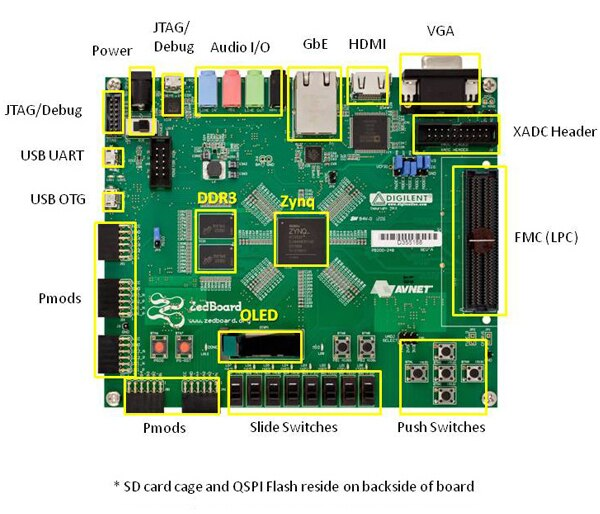
\includegraphics[width = 0.9\textwidth]{ZedBoard-Overlay.jpg}
        \caption{Widok z góry płytki ewaluacyjnej ZedBoard z zaznaczonymi portami \cite{ZedBoard}.}
        \label{fig:ZedBoard_top}
    \end{figure}
    Po uruchomieniu platformy można uruchomić skrypt służący do konfiguracji układu bezpośredniej syntezy cyfrowej. 
    Skrypt posiada kilka poleceń: 
    \begin{itemize}
        \item \textit{help} lub \textit{?} - wyświetla informacje o dostępnych poleceniach,
        \item \textit{connect} - umożliwia połączenie z układem DDS za pomocą portu szeregowego COM,
        \item \textit{prepare} - służy do ustawienie parametrów generowanego sygnału,
        \item \textit{step} - ładuje zadany krok fazowy do układu FPGA,
        \item \textit{load} - ładuje wygenerowany sygnał do pamięci próbek,
        \item \textit{generate} - uruchamia generacje sygnału,
        \item \textit{reset} - przywraca stan początkowy układu DDS,
        \item \textit{stop} - zatrzymuje generacje sygnału, 
        \item \textit{bist} - uruchamia self-test układu DDS, a następnie odbiera raport testu, 
        \item \textit{quit} - zamyka połaczenie z urządzeniem , a następnie kończy działanie programu
    \end{itemize}
    Polecenia pozwalają na proste w obsłudze zarządzanie układem bezpośredniej syntezy cyfrowej. 
    \subsection{Opis poleceń}
        Poniżej zaprezentowano krótki opis poleceń oraz przyjmowane argumenty. W przypadku wprowadzenia polecenia, którego nie 
        ma na liście poleceń, żadne nie zostanie wykonane, a użytkownik zostanie poinformowany o wprowadzeniu błędnej informacji. 
        \subsubsection{Poecenie \textit{help}}
            Wyświetla listę wszystkich poleceń wraz z przyjmowanymi argumentami. 
            Wynik działania zaprezentowano na rysunku \ref{fig:help_output}.
            \begin{figure}[!ht]
                \centering
                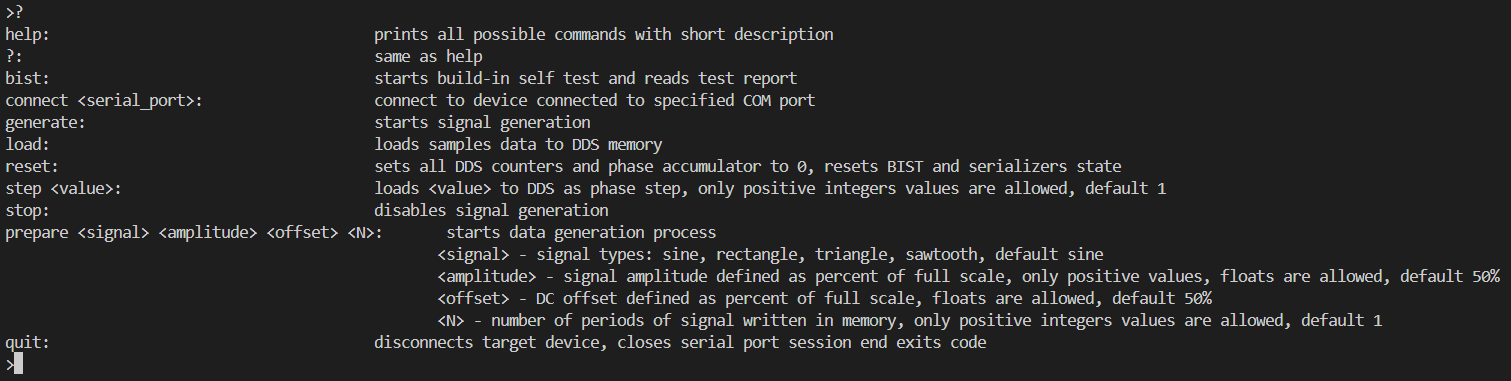
\includegraphics[width = 0.9\textwidth]{help_usage.png}
                \caption{Wynik działania polecenia \textit{help}.}
                \label{fig:help_output}
            \end{figure}
        \subsubsection{Polecenie \textit{connect}}
            Polecenie przyjmuje jeden argument - port szeregowy. Przykładowe wywołanie \textit{connect com1} 
            spowoduje próbę połaczenia z urządzeniem podłaczonym do portu COM1. W przypadku wystąpienia błędu 
            z połaczeniem, użytkownik zostanie poinformowany oraz otrzyma listę dostępnych urządzeń. 
            Jeśli urządzenie nie zostanie znalezione, można wywołać najwyższy numer portu, co spowoduje 
            ponowne wyszukanie urządzeń. W sytuacji, gdy użytkownik wywoła polecenia \textit{connect}, ale nie 
            zdefiniuje portu, zostanie użyty port domyślny - COM1. 
        \subsubsection{Polecenie \textit{prepare}}
            Polecenie przyjmuje 4 argumenty: kształt sygnału, amplitudę wyrażoną w $\%$ pełnego zakresu, offset wyrażony w 
            $\%$ pełnego zakresu oraz liczbę okresów, które zostaną załadowane do pamięci. 
            Skrypt pozwala wygenerować podstawowe przebiegi: 
            \begin{itemize}
                \item sygnał sinusoidalny - \textit{sine},
                \item sygnał prostokątny - \textit{rectangle},
                \item sygnał trójkątny - \textit{triangle},
                \item sygnał piło-kształtny - \textit{sawtooth}
            \end{itemize}
            Inne kształty przebiegów zostaną zaimplementowane w kolejnych wersjach oprogramowania. 
            Dzięki oprogramowaniu, można szybko przygotować próbki, bez obaw o ich rozmieszczenie w pamięci próbek, 
            oraz ich reprezentacje binarną. W przypadku podania błędnych parametrów, zostaną użyte wartości 
            domyślne. Domyślnym sygnałem jest $1$ okres sinusa o amplitudzie $50\ \%$ pełnego zakresu i offsecie 
            wynoszącym $50\ \%$. Jeśli tylko część argumentów jest błędna, pozostałe zostaną wprowadzone prawidłowo. 
            Użytkownik zostanie poinformowany o błędach odpowiednimi komunikatami. Możliwe jest też podanie 
            amplitudy lub offsetu wykraczającego po za zakres. W takiej sytuacji podane wartości zostaną wprowadzone, a 
            użytkownik zostanie poinformowany odpowiednim ostrzeżeniem - nie jest to traktowane jako błąd, gdyż zakłada się, że 
            użytkownik może celowo wygenerować sygnał zniekształcony. Po wygenerowaniu wartości próbek, zostanie wyświetlony 
            wykres z idealnym sygnałem wprowadzonym przez użytkownika oraz sygnał poddany kwantyzacji i ograniczeniu 
            do pełnego zakresu - szczyty sygnału zostaną odpowiednio obcięte do skrajnych wartości, tj. $0$ lub $255$. 
            Liczba okresów sygnału powinna być liczbą całkowitą z zakresu $1 \div 1024$, co odpowiada od $8$ do $8192$ próbek na okres. 
            Wprowadzenie większej liczby okresów będzie skutkowało ostrzeżeniem i zastosowaniem wartości domyślnej.
            Przykład prawidłowego zastosowania polecenia został przedstawiony na rysunku \ref{fig:prepare_correct}, a 
            przykład wprowadzenia błędnych danych na rysunku \ref{fig:prepare_incorrect}. Sygnały wygenerowane na 
            podstawie podanych wartości zostały przedstawione na rysunkach \ref{fig:signal_correct} oraz \ref{fig:signal_incorrect}.
            \begin{figure}[!ht]
                \centering
                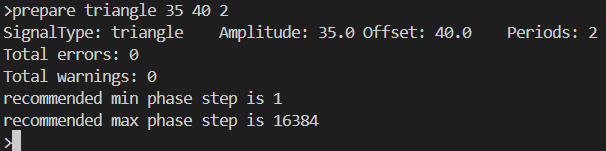
\includegraphics[width = 0.9\textwidth]{correct_prepare.png}
                \caption{Przykład prawidłowego użycia polecenia \textit{prepare}.}
                \label{fig:prepare_correct}
            \end{figure}
            \begin{figure}[!ht]
                \centering
                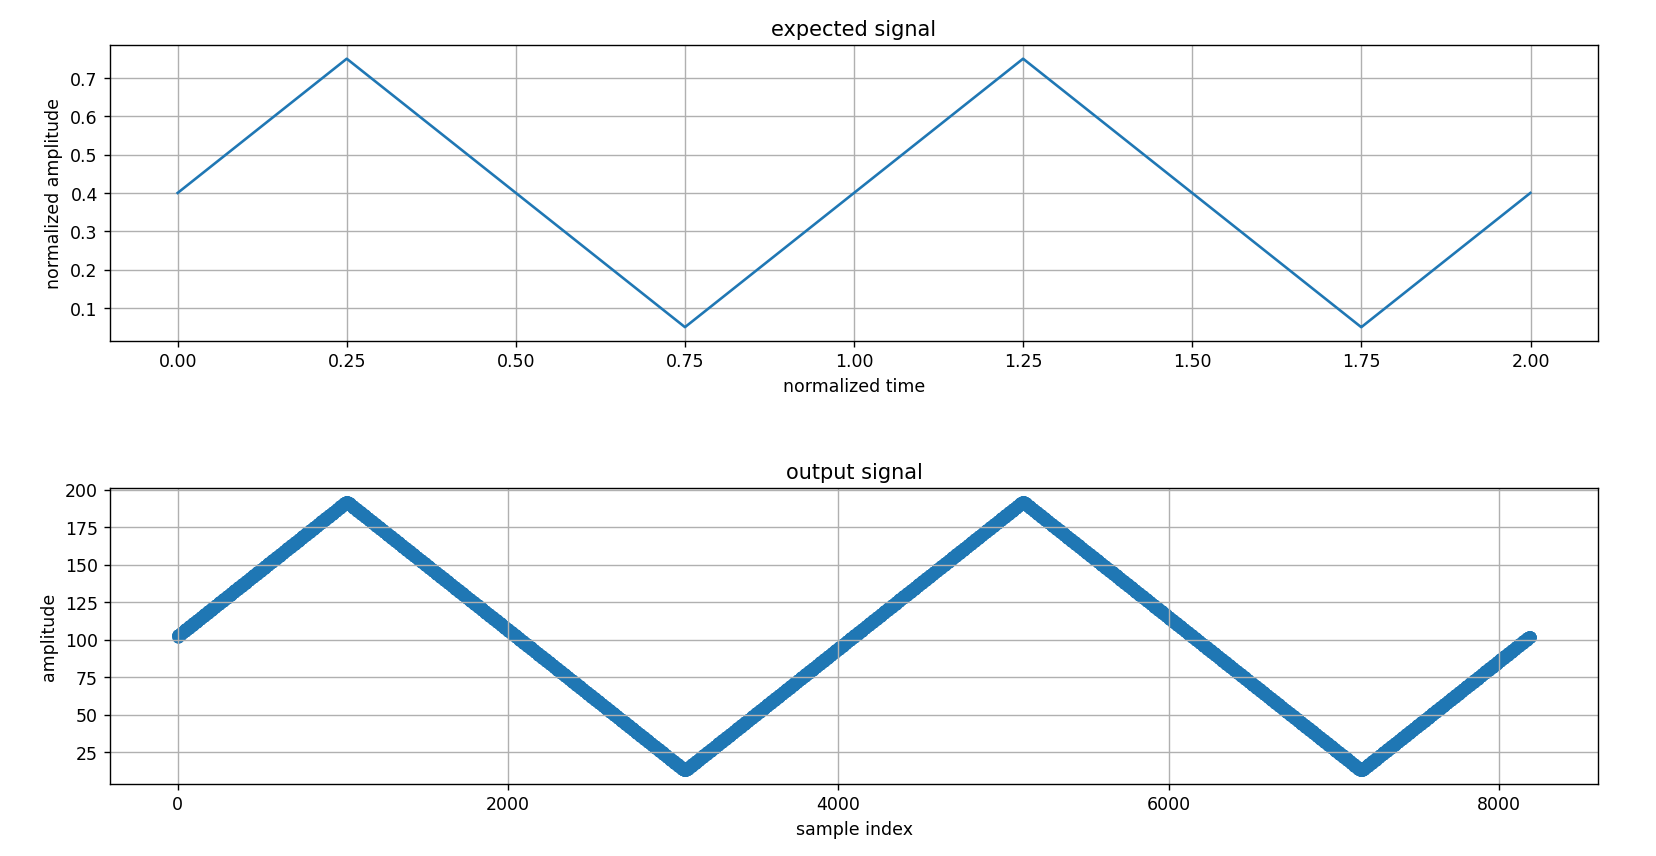
\includegraphics[width = 0.9\textwidth]{correct_signal.png}
                \caption{Przykład prawidłowo wygenerowanego sygnału.}
                \label{fig:signal_correct}
            \end{figure}

            \begin{figure}[!ht]
                \centering
                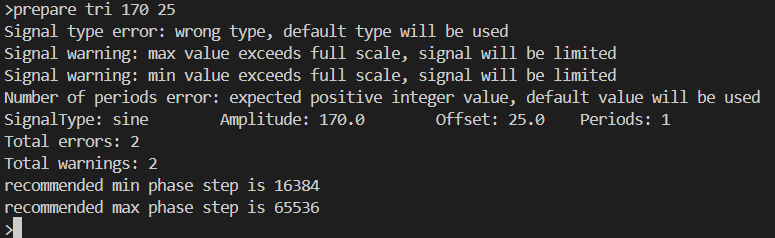
\includegraphics[width = 0.9\textwidth]{incorrect_prepare.png}
                \caption{Przykład błędnego użycia polecenia \textit{prepare} - błędna nazwa sygnału, oraz nie podana liczba okresów.}
                \label{fig:prepare_incorrect}
            \end{figure}
            \begin{figure}[!ht]
                \centering
                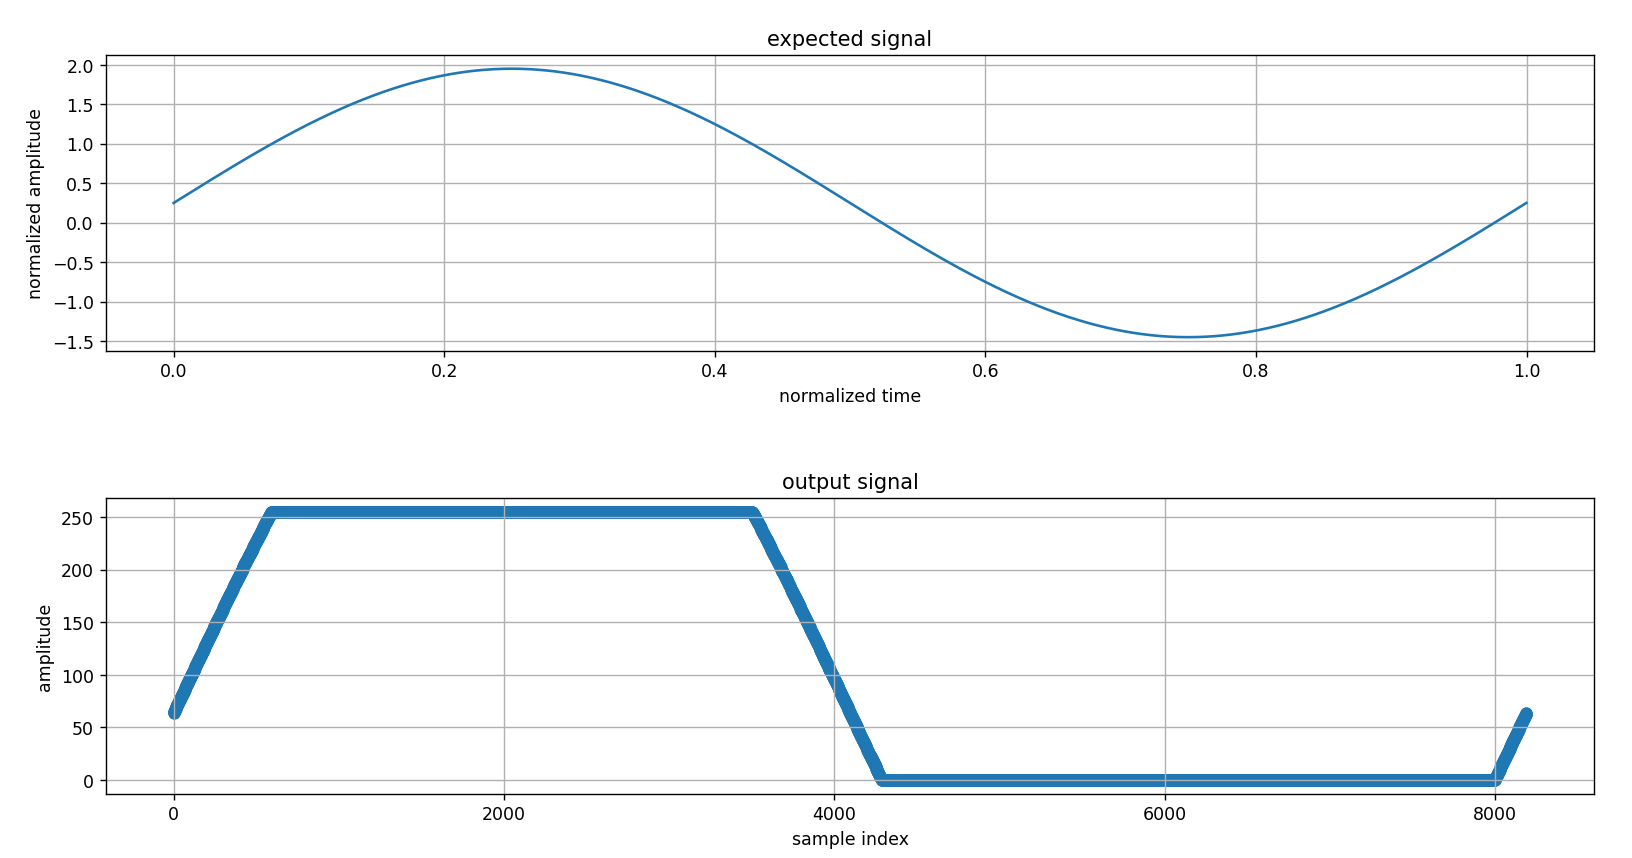
\includegraphics[width = 0.9\textwidth]{incorrect_signal.png}
                \caption{Przykład nieprawidłowo wygenerowanego sygnału - za duża amplituda i offset spowodowały niesymetryczne obcięcie szczytów sinusa (zakładając, że użytkownik chciał otrzymać sygnał bez zniekształceń).}
                \label{fig:signal_incorrect}
            \end{figure}
            
        \subsubsection{Polecenie \textit{step}}
            Polecenie przyjmuje jeden argument - wartość kroku fazowego w postaci dodatniej liczby całkowitej 
            z zakresu $1 \div 65535$ - wartości powyżej $16383$ pozwalają pomijać komórki pamięci - jest to zalecane 
            przy generowaniu szybkich sygnałów. W przypadku podania błędnej wartości lub nie podania żadnej, użytkownik zostanie 
            poinformowany oraz zostanie użyta wartość domyślna wynosząca $1$.
        \subsubsection{Polecenie \textit{load}}
            Wywołanie polecenia powoduje załadownia wygenerowanych danych do pamięci próbek. 
            W przypadku problemów z komunikacją z urządzeniem lub nie wygenerowania danych, 
            użytkownik zostanie poinformowany odpowiednim komunikatem błędu. 
        \subsubsection{Polecenie \textit{generate}}
            Polecenie uruchamia generację sygnału. W przypadku braku komunikacji, 
            użytkownik zostanie poinformowany odpowiednim błędem.
        \subsubsection{Polecenie \textit{reset}}
            Polecenie daje możliwość wyzerowania akumulatora fazy, licznika błędów oraz układów do serializacji danych. 
            W przypadku błędu komunikacji z urządzeniem informuje użytkownika odpowiednim komunikatem błędu. 
        \subsubsection{Polecenie \textit{stop}}
            Zatrzymuje generację sygnału oraz wyprowadza $0$ na wyjściach serializerów. 
            Informuje użytkownika jeśli wystąpi błąd komunikacji. 
        \subsubsection{Polecenie \textit{bist}}
            Polecenie pozwala na przetestowanie poprawności działania układów wyjściowych poprzez serializację i deserializację 
            sygnału pseudolosowego, generowanego wewnątrz układu FPGA. Wynik testu zostaje przekazany użytkownikowi w postaci 
            liczby wektorów testowych, liczby prawidłowo oraz błędnie przetworzonych wektorów. 
            W kolejnych wersjach oprogramowania zostanie zaimplementowana możliwość odczytywania dla jakich 
            wartości wystąpiły błędy w celu analizy wystąpienia potencjalnych uszkodzeń. 
        \subsubsection{Polecenie \textit{quit}}
            Polecenie kończy komunikację z układem FPGA, zamyka otwartą sesję i wyłącza oprogramowanie sterujące. 